\documentclass[a4paper, 10pt]{scrartcl}\usepackage[]{graphicx}\usepackage[]{color}
%% maxwidth is the original width if it is less than linewidth
%% otherwise use linewidth (to make sure the graphics do not exceed the margin)
\makeatletter
\def\maxwidth{ %
  \ifdim\Gin@nat@width>\linewidth
    \linewidth
  \else
    \Gin@nat@width
  \fi
}
\makeatother

\definecolor{fgcolor}{rgb}{0.345, 0.345, 0.345}
\newcommand{\hlnum}[1]{\textcolor[rgb]{0.686,0.059,0.569}{#1}}%
\newcommand{\hlstr}[1]{\textcolor[rgb]{0.192,0.494,0.8}{#1}}%
\newcommand{\hlcom}[1]{\textcolor[rgb]{0.678,0.584,0.686}{\textit{#1}}}%
\newcommand{\hlopt}[1]{\textcolor[rgb]{0,0,0}{#1}}%
\newcommand{\hlstd}[1]{\textcolor[rgb]{0.345,0.345,0.345}{#1}}%
\newcommand{\hlkwa}[1]{\textcolor[rgb]{0.161,0.373,0.58}{\textbf{#1}}}%
\newcommand{\hlkwb}[1]{\textcolor[rgb]{0.69,0.353,0.396}{#1}}%
\newcommand{\hlkwc}[1]{\textcolor[rgb]{0.333,0.667,0.333}{#1}}%
\newcommand{\hlkwd}[1]{\textcolor[rgb]{0.737,0.353,0.396}{\textbf{#1}}}%
\let\hlipl\hlkwb

\usepackage{framed}
\makeatletter
\newenvironment{kframe}{%
 \def\at@end@of@kframe{}%
 \ifinner\ifhmode%
  \def\at@end@of@kframe{\end{minipage}}%
  \begin{minipage}{\columnwidth}%
 \fi\fi%
 \def\FrameCommand##1{\hskip\@totalleftmargin \hskip-\fboxsep
 \colorbox{shadecolor}{##1}\hskip-\fboxsep
     % There is no \\@totalrightmargin, so:
     \hskip-\linewidth \hskip-\@totalleftmargin \hskip\columnwidth}%
 \MakeFramed {\advance\hsize-\width
   \@totalleftmargin\z@ \linewidth\hsize
   \@setminipage}}%
 {\par\unskip\endMakeFramed%
 \at@end@of@kframe}
\makeatother

\definecolor{shadecolor}{rgb}{.97, .97, .97}
\definecolor{messagecolor}{rgb}{0, 0, 0}
\definecolor{warningcolor}{rgb}{1, 0, 1}
\definecolor{errorcolor}{rgb}{1, 0, 0}
\newenvironment{knitrout}{}{} % an empty environment to be redefined in TeX

\usepackage{alltt}  %article

% Permet l'encodage avec le Unicode Transformation Format-8-bit
\usepackage[utf8]{inputenc}
% Permet la gestion des caractères accentués ainsi que la stabilité des impressions en P.D.F.
\usepackage[T1]{fontenc}
% Permet la stabilisation de l'écriture
\usepackage{lmodern}
% Permet d'utiliser les liens hypertexte sans altérer la bibliothèque KOMA
\usepackage{scrhack}
\KOMAoptions{hyperref=false}
% Utilise les règles gramaticales françaises
\usepackage[french]{babel}

%Utilise les règles typographique de la bibliothéques KOMA
\setkomafont{author}{\scshape}
%\usepackage{blindtext}

% Package pour avoir plus d'arguments dans ses commandes.
\usepackage{xargs}

%Bibliothèque mathématiques pour la police.
\usepackage{amsfonts}
%Bibliothèques mathématiques générale.
\usepackage{amsmath}
\usepackage{amssymb}
%Pour appliquer \mathbb à des nombres
\usepackage{bbm}
%Package pour l'indexation de matrices
\usepackage{blkarray}
%\usepackage{dsfont}
%Bibliothèque pour l'affichage de nombre avec la typographie définie
\usepackage{numprint}
\newcommand{\np}[1]{\numprint{#1}}
% Pour la notation scientifique
\usepackage{siunitx}
\sisetup{locale= FR,exponent-product=.}
\DeclareSIUnit\year{ann\'{e}ee}
%Positionnement des images
\usepackage{float}
\usepackage{subcaption}
%Utilisation des couleurs
\usepackage{xcolor}
% Package pour le soulignement
\usepackage{color,soulutf8}
\setulcolor{red}
% Package pour les annotations
\usepackage{todonotes}
%\usepackage[pygments]{pythontex} % Pour utiliser Python
%\usepackage{fvextra} % Utile pour la mise en forme du code source inséré
%Package pour la programmation
\usepackage{listings}
% Package pour les scripts en R
\lstset{language=R,
    basicstyle=\small\ttfamily,
    stringstyle=\color{DarkGreen},
    otherkeywords={0,1,2,3,4,5,6,7,8,9},
    morekeywords={TRUE,FALSE},
    deletekeywords={data,frame,length,as,character},
    keywordstyle=\color{blue},
    commentstyle=\color{DarkGreen},
    }

%Définition de couleurs:
\definecolor{bleudefrance}{rgb}{.19, .55, .91}
\definecolor{pakistangreen}{rgb}{.0, .4, .0}
\definecolor{rossocorsa}{rgb}{0.83, 0.0, 0.0}
\definecolor{persimmon}{rgb}{0.93, 0.35, 0.0}
% Annotation auteur
\newcommand{\Moi}[1]{\todo[color = teal!40]{#1}}
\newcommand{\Cnsl}[1]{\todo[color = pakistangreen!40]{#1}}
\newcommand{\MeG}[1]{\todo[color = rossocorsa!40]{#1}}
%Notation récurrante:
\newcommandx{\hb}[1]{\widehat{\beta_{#1}}}
\newcommandx{\prth}[3]{\left( #1 \right)_{1\leq #2 \leq #3}}
% Encadrement des résultats
\newcommand{\enc}[1]{\fcolorbox{rossocorsa}{white}{#1}}
\newcommand{\encB}[1]{\fcolorbox{bleudefrance}{white}{#1}}
\newcommand{\encV}[1]{\fcolorbox{pakistangreen}{white}{#1}}
\newcommand{\encN}[1]{\fcolorbox{black}{white}{#1}}
% Soulignement couleur
\newcommandx{\sN}[1]{\setulcolor{black}\ul{#1}}
\newcommandx{\sR}[1]{\setulcolor{rossocorsa}\ul{#1}}
\newcommandx{\sB}[1]{\setulcolor{bleudefrance}\ul{#1}}
\newcommandx{\sV}[1]{\setulcolor{pakistangreen}\ul{#1}}
\newcommandx{\sT}[1]{\setulcolor{teal}\ul{#1}}
\newcommandx{\sO}[1]{\setulcolor{persimmon}\ul{#1}}
% Text de couleur
\newcommandx{\tR}[1]{\textcolor{rossocorsa}{#1}}
\newcommandx{\tB}[1]{\textcolor{bleudefrance}{#1}}
\newcommandx{\tV}[1]{\textcolor{pakistangreen}{#1}}
\newcommandx{\tT}[1]{\textcolor{teal}{#1}}
\newcommandx{\tO}[1]{\textcolor{persimmon}{#1}}
% Écriture intervalle
\newcommandx{\inter}[2]{\left[\![#1, #2]\!\right]}
% Écriture intégrale
\newcommand{\Su}[2]{\int\limits_#1^#2}
% Écriture somme sigma
\newcommand{\su}[2]{\sum\limits_#1^#2}
% Écriture P(X)
\newcommandx{\prob}[1]{\mathbb{P}\left(#1\right)}
% Écriture P({X})
\newcommandx{\Prob}[1]{\mathbb{P}\left(\left\{#1 \right\}\right)}
% Écriture P_{\{Y\}}({X})
\newcommandx{\ProbC}[2]{\mathbb{P}_{\left\{#1\right\}}\left(\left\{#2\right\}\right)}
% Ecriture Esperance et Variance
\newcommandx{\E}[1]{\mathbb{E}\left(#1\right)}
\newcommandx{\V}[1]{\mathbb{V}\left(#1\right)}
%Symbole de la norme
\newcommandx{\norm}[1]{\left\lVert#1\right\rVert}

\title{Titre}
\author{Siger}
\IfFileExists{upquote.sty}{\usepackage{upquote}}{}
\begin{document}

\paragraph{8.}
\begin{itemize}
	\item[(a)] We perform a simple linear regression with \emph{
		mpg} as the response and \emph{horsepower} as a 
		predictor. Here the results:
\begin{knitrout}
\definecolor{shadecolor}{rgb}{0.969, 0.969, 0.969}\color{fgcolor}\begin{kframe}
\begin{alltt}
\hlkwd{library}\hlstd{(MASS)}
\hlkwd{library}\hlstd{(ISLR)}
\hlkwd{library}\hlstd{(car)}
\hlstd{lm.fit} \hlkwb{=} \hlkwd{lm}\hlstd{(mpg}\hlopt{~}\hlstd{horsepower,} \hlkwc{data}\hlstd{=Auto)}
\hlkwd{summary}\hlstd{(lm.fit)}
\end{alltt}
\begin{verbatim}
## 
## Call:
## lm(formula = mpg ~ horsepower, data = Auto)
## 
## Residuals:
##      Min       1Q   Median       3Q      Max 
## -13.5710  -3.2592  -0.3435   2.7630  16.9240 
## 
## Coefficients:
##              Estimate Std. Error t value Pr(>|t|)    
## (Intercept) 39.935861   0.717499   55.66   <2e-16 ***
## horsepower  -0.157845   0.006446  -24.49   <2e-16 ***
## ---
## Signif. codes:  0 '***' 0.001 '**' 0.01 '*' 0.05 '.' 0.1 ' ' 1
## 
## Residual standard error: 4.906 on 390 degrees of freedom
## Multiple R-squared:  0.6059,	Adjusted R-squared:  0.6049 
## F-statistic: 599.7 on 1 and 390 DF,  p-value: < 2.2e-16
\end{verbatim}
\end{kframe}
\end{knitrout}
We can observe that there is a relationship between the predictor and 
the response
		\begin{itemize}
			\item[i.] We can observe, that the \emph{
				p-value} is very low so we can believe
				that there is a relationship between
				the predictor and the response.
			\item[ii.] The RSE equal to $4.906$ on $390$
				degrees of freedom and $R^{2}=60.59\%$
				that shows the relationship is a priori
				strong.
			\item[iii.] The slope of this simple linear
				regression is positive thus the
				relationship between the predictor and
				the response is positive.
			\item[iv.]
\begin{knitrout}
\definecolor{shadecolor}{rgb}{0.969, 0.969, 0.969}\color{fgcolor}\begin{kframe}
\begin{alltt}
\hlkwd{attach}\hlstd{(Auto)}
\hlcom{#To get confidence interval:}
\hlkwd{predict}\hlstd{(lm.fit,} \hlkwd{data.frame}\hlstd{(}\hlkwc{horsepower}\hlstd{=}\hlnum{98}\hlstd{),} \hlkwc{interval}\hlstd{=}\hlstr{"confidence"}\hlstd{)}
\end{alltt}
\begin{verbatim}
##        fit      lwr      upr
## 1 24.46708 23.97308 24.96108
\end{verbatim}
\begin{alltt}
\hlcom{#To get prediction interval:}
\hlkwd{predict}\hlstd{(lm.fit,} \hlkwd{data.frame}\hlstd{(}\hlkwc{horsepower}\hlstd{=}\hlnum{98}\hlstd{),} \hlkwc{interval}\hlstd{=}\hlstr{"prediction"}\hlstd{)}
\end{alltt}
\begin{verbatim}
##        fit     lwr      upr
## 1 24.46708 14.8094 34.12476
\end{verbatim}
\end{kframe}
\end{knitrout}
				So the associated $95\%$ confidence and
				predictive intervals are respectively
				equal to: $[23.97, 24.96]$ and $[14.81,
				34.12]$
		\end{itemize}
	\item[(b)] We will plot the response and the predictor:
\begin{knitrout}
\definecolor{shadecolor}{rgb}{0.969, 0.969, 0.969}\color{fgcolor}\begin{kframe}
\begin{alltt}
\hlcom{#To plot }
\hlkwd{plot}\hlstd{(horsepower, mpg,} \hlkwc{col}\hlstd{=}\hlstr{'red'}\hlstd{,} \hlkwc{pch}\hlstd{=}\hlstr{'+'}\hlstd{)}
\hlkwd{abline}\hlstd{(lm.fit,} \hlkwc{lwd}\hlstd{=}\hlnum{3}\hlstd{,} \hlkwc{col}\hlstd{=}\hlstr{'green'}\hlstd{)}
\end{alltt}
\end{kframe}\begin{figure}[H]
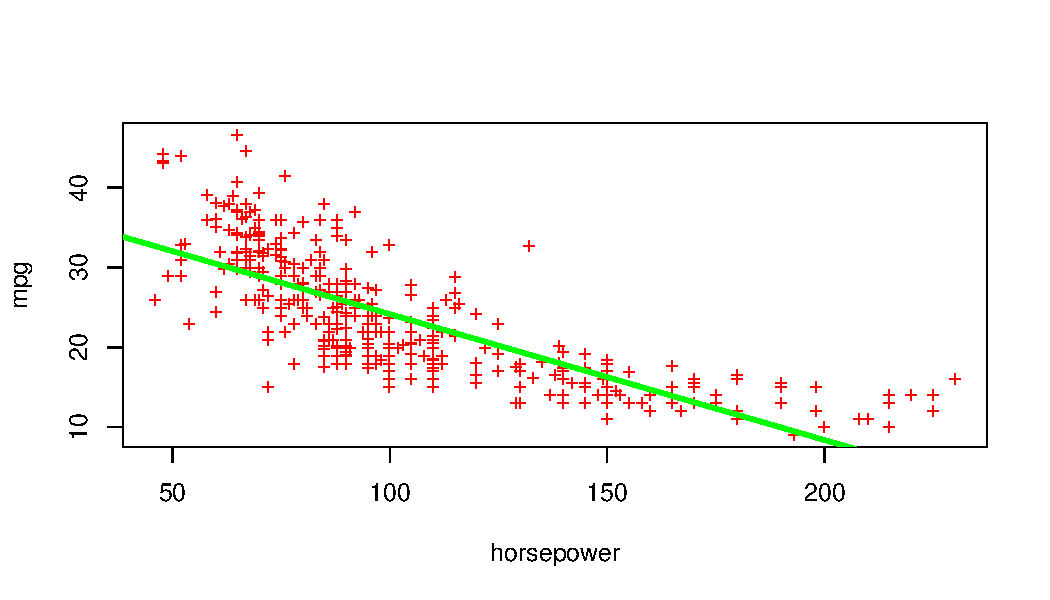
\includegraphics[width=\maxwidth]{figure/p1b-1} \caption[The response and the predictor]{The response and the predictor.}\label{fig:p1b}
\end{figure}


\end{knitrout}
	\item[(c)] As we are in simple regression settings to check
		if there is a \emph{Non-linerity of the Data} for this
		we plot simply residual errors vs predictor:
\begin{knitrout}
\definecolor{shadecolor}{rgb}{0.969, 0.969, 0.969}\color{fgcolor}\begin{kframe}
\begin{alltt}
\hlkwd{plot}\hlstd{(horsepower,} \hlkwd{residuals}\hlstd{(lm.fit),} \hlkwc{type}\hlstd{=}\hlstr{'o'}\hlstd{,} \hlkwc{col}\hlstd{=}\hlstr{'blue'}\hlstd{)}
\end{alltt}
\end{kframe}\begin{figure}[H]
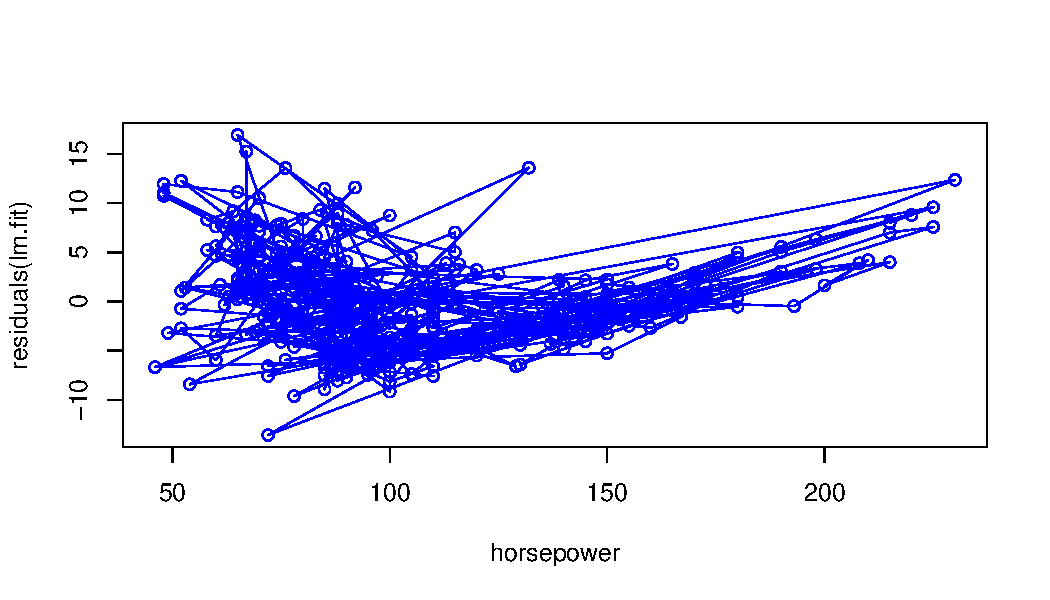
\includegraphics[width=\maxwidth]{figure/p2b-1} \caption[Residuals errors vs predictor]{Residuals errors vs predictor.}\label{fig:p2b}
\end{figure}


\end{knitrout}
		After this we check if it exists correlation of errors
		terms, ploting Residuals vs observation number:
\begin{knitrout}
\definecolor{shadecolor}{rgb}{0.969, 0.969, 0.969}\color{fgcolor}\begin{kframe}
\begin{alltt}
\hlkwd{plot}\hlstd{(}\hlkwd{residuals}\hlstd{(lm.fit),} \hlkwc{type}\hlstd{=}\hlstr{'o'}\hlstd{,} \hlkwc{col}\hlstd{=}\hlstr{'red'}\hlstd{)}
\hlkwd{title}\hlstd{(}\hlkwc{xlab}\hlstd{=}\hlstr{'Observation number'}\hlstd{)}
\end{alltt}
\end{kframe}\begin{figure}[H]
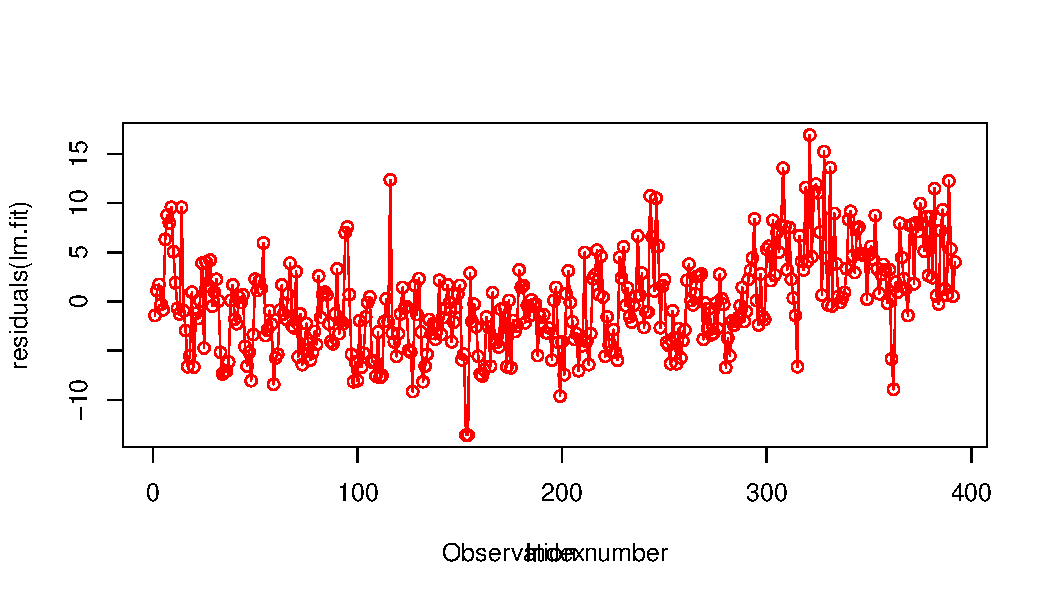
\includegraphics[width=\maxwidth]{figure/p3b-1} \caption[Residuals vs observation number]{Residuals vs observation number.}\label{fig:p3b}
\end{figure}


\end{knitrout}
We do not observe pattern in those plots.\\The residual errors stay
confined so there is no \emph{Non-constant variance of error terms}
issues. We do not see neither \emph{Outliers} or \emph{High leverage
points}. Finaly as a simple regression there is no matter of \emph{
Colinearity}
\end{itemize}
\paragraph{9.}
\begin{itemize}
	\item[(a)] Here a scatterplot matrix including all variables:
\begin{knitrout}
\definecolor{shadecolor}{rgb}{0.969, 0.969, 0.969}\color{fgcolor}\begin{kframe}
\begin{alltt}
\hlkwd{pairs}\hlstd{(Auto)}
\end{alltt}
\end{kframe}\begin{figure}[H]
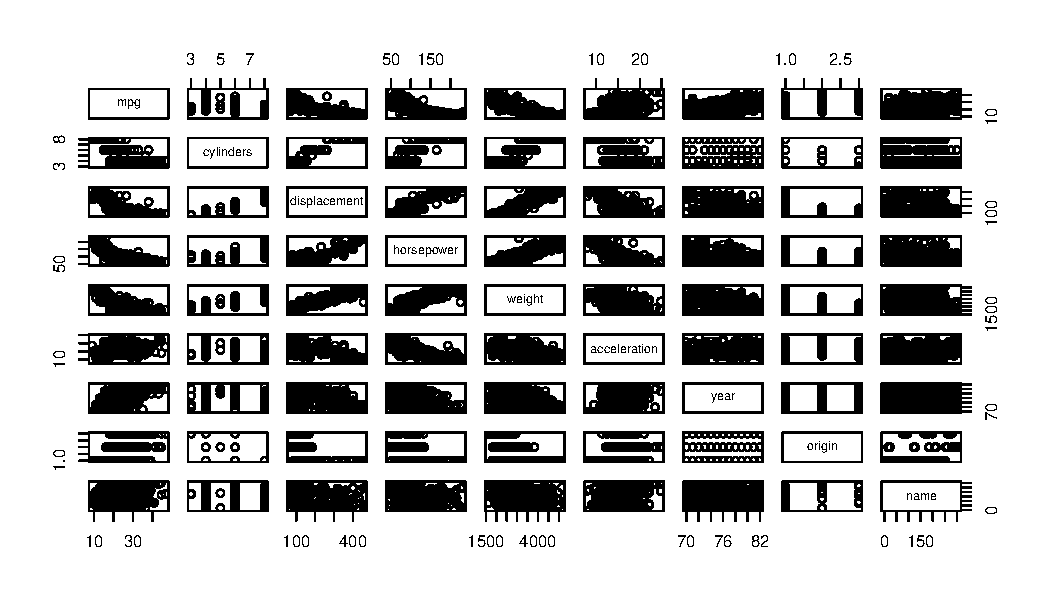
\includegraphics[width=\maxwidth]{figure/p4b-1} \caption[Scatterplot matrix]{Scatterplot matrix.}\label{fig:p4b}
\end{figure}


\end{knitrout}
	\item[(b)] For the matrix of correlation:
\begin{knitrout}
\definecolor{shadecolor}{rgb}{0.969, 0.969, 0.969}\color{fgcolor}\begin{kframe}
\begin{alltt}
\hlstd{Table} \hlkwb{=} \hlkwd{data.frame}\hlstd{(Auto)}
\hlkwd{cor}\hlstd{(Table[,} \hlopt{-}\hlnum{9}\hlstd{])}
\end{alltt}
\begin{verbatim}
##                     mpg  cylinders displacement horsepower     weight
## mpg           1.0000000 -0.7776175   -0.8051269 -0.7784268 -0.8322442
## cylinders    -0.7776175  1.0000000    0.9508233  0.8429834  0.8975273
## displacement -0.8051269  0.9508233    1.0000000  0.8972570  0.9329944
## horsepower   -0.7784268  0.8429834    0.8972570  1.0000000  0.8645377
## weight       -0.8322442  0.8975273    0.9329944  0.8645377  1.0000000
## acceleration  0.4233285 -0.5046834   -0.5438005 -0.6891955 -0.4168392
## year          0.5805410 -0.3456474   -0.3698552 -0.4163615 -0.3091199
## origin        0.5652088 -0.5689316   -0.6145351 -0.4551715 -0.5850054
##              acceleration       year     origin
## mpg             0.4233285  0.5805410  0.5652088
## cylinders      -0.5046834 -0.3456474 -0.5689316
## displacement   -0.5438005 -0.3698552 -0.6145351
## horsepower     -0.6891955 -0.4163615 -0.4551715
## weight         -0.4168392 -0.3091199 -0.5850054
## acceleration    1.0000000  0.2903161  0.2127458
## year            0.2903161  1.0000000  0.1815277
## origin          0.2127458  0.1815277  1.0000000
\end{verbatim}
\end{kframe}
\end{knitrout}
	\item[(c)]We use multiple linear regression with mpg and the 
		predictors
\begin{knitrout}
\definecolor{shadecolor}{rgb}{0.969, 0.969, 0.969}\color{fgcolor}\begin{kframe}
\begin{alltt}
\hlstd{lm.fit} \hlkwb{=} \hlkwd{lm}\hlstd{(mpg}\hlopt{~}\hlstd{.}\hlopt{-}\hlstd{name,} \hlkwc{data}\hlstd{=Auto)}
\hlkwd{summary}\hlstd{(lm.fit)}
\end{alltt}
\begin{verbatim}
## 
## Call:
## lm(formula = mpg ~ . - name, data = Auto)
## 
## Residuals:
##     Min      1Q  Median      3Q     Max 
## -9.5903 -2.1565 -0.1169  1.8690 13.0604 
## 
## Coefficients:
##                Estimate Std. Error t value Pr(>|t|)    
## (Intercept)  -17.218435   4.644294  -3.707  0.00024 ***
## cylinders     -0.493376   0.323282  -1.526  0.12780    
## displacement   0.019896   0.007515   2.647  0.00844 ** 
## horsepower    -0.016951   0.013787  -1.230  0.21963    
## weight        -0.006474   0.000652  -9.929  < 2e-16 ***
## acceleration   0.080576   0.098845   0.815  0.41548    
## year           0.750773   0.050973  14.729  < 2e-16 ***
## origin         1.426141   0.278136   5.127 4.67e-07 ***
## ---
## Signif. codes:  0 '***' 0.001 '**' 0.01 '*' 0.05 '.' 0.1 ' ' 1
## 
## Residual standard error: 3.328 on 384 degrees of freedom
## Multiple R-squared:  0.8215,	Adjusted R-squared:  0.8182 
## F-statistic: 252.4 on 7 and 384 DF,  p-value: < 2.2e-16
\end{verbatim}
\end{kframe}
\end{knitrout}
	\begin{itemize}
		\item[i.] The \emph{F-statistic} is a means to compute
			hypothesis test to know if there is or not a
			relationship between the response and the 
			predictors. When $F-statistic$ takes a value
			close to $1$ then there is not relationship,
			but here \emph{F-statistic} equals to $252.4$
			on the $7$ predictors that are the most 
			significant.
		\item[ii.] Regarding the \emph{p-value} associated
			with \emph{F-statistic} the most significant
			predictors are: weight, year, origin and
			displacement.
		\item[iii.] The year coefficient means that in $10$
			years the distance traveled growth of $75$
			miles per gallon.
	\end{itemize}
	\item[(d)] Recall that main problems that we can encountered
		are: \emph{Non-linerity of the Data, Correlation of
		error terms, Non-constant variance of error terms,
		Outliers, High-leverage points, and Colinearity}.
		\begin{itemize}
			\item[Non-linerity] It suffices to plot 
				residual errors vs the predicted 
				response
\begin{knitrout}
\definecolor{shadecolor}{rgb}{0.969, 0.969, 0.969}\color{fgcolor}\begin{kframe}
\begin{alltt}
\hlstd{y_predict} \hlkwb{=} \hlkwd{predict}\hlstd{(lm.fit)}
\hlkwd{plot}\hlstd{(y_predict,} \hlkwd{residuals}\hlstd{(lm.fit),} \hlkwc{type}\hlstd{=}\hlstr{'o'}\hlstd{,} \hlkwc{col}\hlstd{=}\hlstr{'blue'}\hlstd{)}
\end{alltt}
\end{kframe}\begin{figure}[H]
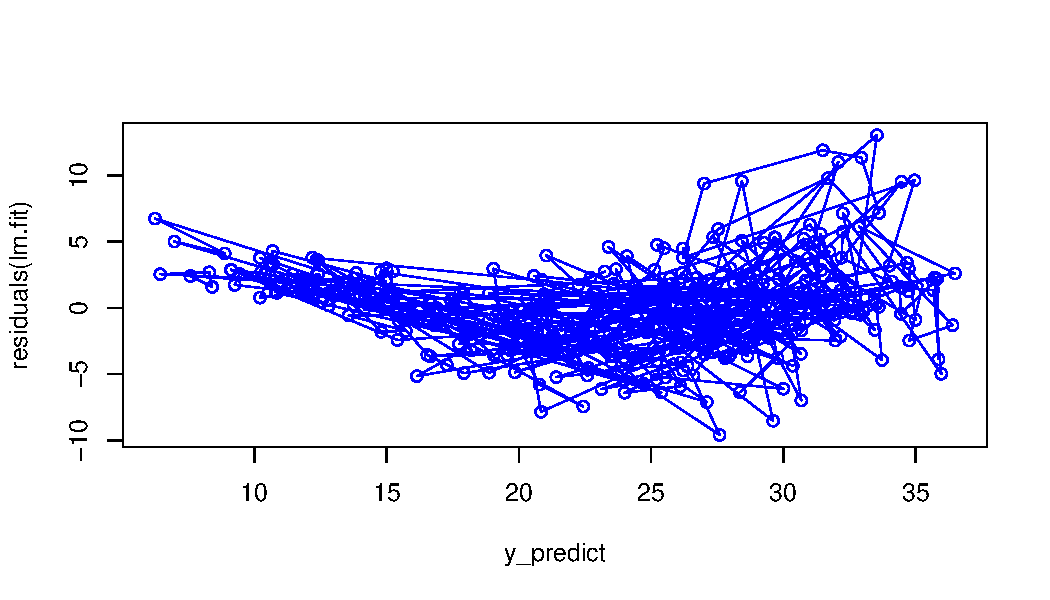
\includegraphics[width=\maxwidth]{figure/p6b-1} \caption[Residuals vs the predicted response]{Residuals vs the predicted response.}\label{fig:p6b}
\end{figure}


\end{knitrout}
We do not identify any pattern in the Residuals vs the predicted
response plot
			\item[Colinearity of error terms] We plot 
				residuals vesus observation:
\begin{knitrout}
\definecolor{shadecolor}{rgb}{0.969, 0.969, 0.969}\color{fgcolor}\begin{kframe}
\begin{alltt}
\hlkwd{plot}\hlstd{(}\hlkwd{residuals}\hlstd{(lm.fit),} \hlkwc{type}\hlstd{=}\hlstr{'o'}\hlstd{,} \hlkwc{col}\hlstd{=}\hlstr{'red'}\hlstd{)}
\end{alltt}
\end{kframe}\begin{figure}[H]
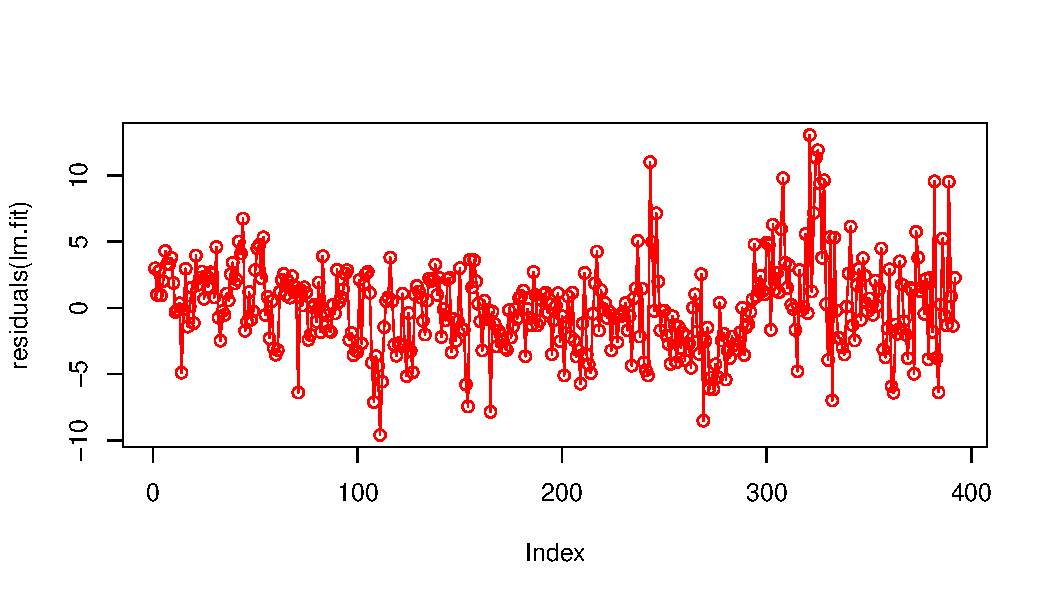
\includegraphics[width=\maxwidth]{figure/p7b-1} \caption[Residuals vs observation number]{Residuals vs observation number.}\label{fig:p7b}
\end{figure}


\end{knitrout}
				This time we observe that residual 
				values increase with observation,
				we suspect a correlation in the error
				terms.
			\item[Non-constant variance of error terms ] We
				can observe that the residual values
				tend to stay confined between $5$ and
				$-5$.
			\item[Non-linerity]
			\item[Non-linerity]
			\item[Non-linerity]
		\end{itemize}
	\item[(e)]
	\item[(f)]
\end{itemize}
\end{document}
